%% ++++++++++++++++++++++++++++++++++++++++++++++++++++++++++++
%% Hauptdatei, Wurzel des Dokuments
%% ++++++++++++++++++++++++++++++++++++++++++++++++++++++++++++

% Headerfeld, Typ des Dokumentes, einzubindende Packages.
% Hier bei Bedarf Änderungen vornehmen.
\documentclass
[   twoside=false,     % Einseitiger oder zweiseitiger Druck?
    fontsize=12pt,     % Bezug: 12-Punkt Schriftgröße
    DIV=15,            % Randaufteilung, siehe Dokumentation "KOMA"-Script
    BCOR=17mm,         % Bindekorrektur: Innen 17mm Platz lassen. Copyshop-getestet.
%    headsepline,
    headsepline,  % Unter Kopfzeile Trennlinie (aus: headnosepline)
    footsepline,  % Über Fußzeile Trennlinie (aus: footnosepline)
    open=right,        % Neue Kapitel im zweiseitigen Druck rechts beginnen lassen
    paper=a4,          % Seitenformat A4
    abstract=true,     % Abstract einbinden
    listof=totoc,      % Div. Verzeichnisse ins Inhaltsverzeichnis aufnehmen
    bibliography=totoc,% Literaturverzeichnis ins Inhaltsverzeichnis aufnehmen
    titlepage,         % Titelseite aktivieren
    headinclude=true,  % Seiten-Head in die Satzspiegelberechnung mit einbeziehen
    footinclude=false, % Seiten-Foot nicht in die Satzspiegelberechnung mit einbeziehen
    numbers=noenddot   % Gliederungsnummern ohne abschließenden Punkt darstellen
]   {scrreprt}         % Dokumentenstil: "Report" aus dem KOMA-Skript-Paket

\usepackage[active]{srcltx}
%\usepackage[activate=normal]{pdfcprot} % Optischer Randausgleich -> pdflatex!
\usepackage{ifthen}
\usepackage[ngerman]{babel}   % Neue Deutsche Rechtschreibung
%\usepackage[latin1]{inputenc} % Zeichencodierung nach ISO-8859-1
\usepackage[utf8]{inputenc}   %	Zeichencodierung nach UTF-8 (Unicode)
\usepackage[T1]{fontenc}
%\usepackage{ae} % obsolet und durch lmodern ersetzt
\usepackage{lmodern}
\usepackage[T1]{url}
\usepackage[final]{graphicx}
\RequirePackage{scrlfile}
\ReplacePackage{scrpage2}{scrlayer-scrpage}
% old: \usepackage[automark]{scrpage2}
\usepackage[automark]{scrlayer-scrpage}
\usepackage{setspace}
%\usepackage[first,light]{draftcopy} % Für Probedruck
\usepackage[plainpages=false,pdfpagelabels,hypertexnames=false]{hyperref}

% Tiefe der Kapitelnummerierung beeinflussen
\setcounter{secnumdepth}{3} % Tiefe der Nummerierung
\setcounter{tocdepth}{3}    % Tiefe des Inhaltsverzeichnisses

% Hier in die zweite geschweifte Klammer jeweils
% die persönlichen Daten und das Thema der Arbeit eintragen:
\newcommand{\artderausarbeitung}{Bachelorarbeit}
\newcommand{\namedesautors}{Max Mustermann}
\newcommand{\themaderarbeit}{Anfertigung einer Ausarbeitung mit \LaTeX}

% PDF Metadaten definieren
\hypersetup{
   pdftitle={\themaderarbeit},
   pdfsubject={\artderausarbeitung},
   pdfauthor={\namedesautors},
   pdfkeywords={\artderausarbeitung; TU-Ilmenau; Kommunikationsnetze;}}


% Abkürzungsverzeichnis beeinflussen. Hier nichts ändern!
\usepackage[intoc]{nomencl}
  \AtBeginDocument{\setlength{\nomlabelwidth}{.25\columnwidth}}
  \let\abbrev\nomenclature
  \renewcommand{\nomname}{Abkürzungsverzeichnis und Formelzeichen}
  \renewcommand{\nomlabel}[1]{#1 \dotfill}
  \setlength{\nomitemsep}{-\parsep}
  \makenomenclature

\usepackage[normalem]{ulem}
  \newcommand{\markup}[1]{\textbf{#1}}

% Seitenlayout festlegen. Hier nichts ändern!
\pagestyle{scrplain}
\ihead[]{\headmark}
\ohead[]{\pagemark}
\chead[]{}
\ifoot[]{}
\ofoot[]{\scriptsize \artderausarbeitung\ \namedesautors}
\cfoot[]{}
\renewcommand{\titlepagestyle}{scrheadings}
\renewcommand{\partpagestyle}{scrheadings}
\renewcommand{\chapterpagestyle}{scrheadings}
\renewcommand{\indexpagestyle}{scrheadings}

% Abschnittsweise Nummerierung anstatt fortlaufend. Hier nichts ändern!
\makeatletter
\@addtoreset{equation}{chapter}
\@addtoreset{figure}{chapter}
\@addtoreset{table}{chapter}
\renewcommand\theequation{\thechapter.\@arabic\c@equation}
\renewcommand\thefigure{\thechapter.\@arabic\c@figure}
\renewcommand\thetable{\thechapter.\@arabic\c@table}
\makeatother

% Quelltextrahmen, klein. Hier nichts ändern!
\newsavebox{\inhaltkl}
\def\rahmenkl{\sbox{\inhaltkl}\bgroup\small\renewcommand{\baselinestretch}{1}\vbox\bgroup\hsize\textwidth}
\def\endrahmenkl{\par\vskip-\lastskip\egroup\egroup\fboxsep3mm%
\framebox[\textwidth][l]{\usebox{\inhaltkl}}}

% Quelltextrahmen, normale Groesse. Hier nichts ändern!
\newsavebox{\inhalt}
\def\rahmen{\sbox{\inhalt}\bgroup\renewcommand{\baselinestretch}{1}\vbox\bgroup\hsize\textwidth}
\def\endrahmen{\par\vskip-\lastskip\egroup\egroup\fboxsep3mm%
\framebox[\textwidth][l]{\usebox{\inhalt}}}

% Trennvorschläge für falsch getrennte Wörter.
% Wird häufig bei eingedeutschen Wörtern benötigt, da LaTeX hierbei
% gerne falsch trennt. Alternativ kann auch im Fliesstext ein
% Trennvorschlag per "\-" hinterlegt werden, bspw.:
% Die Hard\-ware besteht aus A und B.
\hyphenation{
Hard-ware
}

% Sonstige Befehlsdefinitionen hier ablegen.
\newcommand{\entspricht}{\stackrel{\wedge}{=}}

% Tabellenspaltendefinitionen mit fester Breite --> somit Zeilenumbruch innerhalb einer Zelle möglich
% aus http://www.torsten-schuetze.de/tex/tabsatz-2004.pdf
\usepackage{array, booktabs}
\newcolumntype{f}{>{$}l<{$}}
\newcolumntype{n}{>{\raggedright}l}
\newcolumntype{N}{>{\scriptsize}l}
\newcolumntype{v}[1]{>{\raggedright\hspace{0pt}}m{#1}}
\newcolumntype{V}[1]{>{\scriptsize\raggedright\hspace{0pt}}m{#1}}
\newcolumntype{Z}[1]{>{\raggedright\centering}m{#1}}
\newcolumntype{k}[1]{>{\raggedright}p{#1}}
% ergibt Tabllenspalte fester Breite, linksbündig
% Umbruch innerhalb der Zelle mit \\, neue Tabellezeile mit \tabularnewline
% \addlinespace für Gruppentrennung (aus \texttt{booktabs.sty})


\begin{document}
\onehalfspacing
%% ++++++++++++++++++++++++++++++++++++++++++++++++++++++++++++
%% Hauptdatei, Wurzel des Dokuments
%% ++++++++++++++++++++++++++++++++++++++++++++++++++++++++++++
%
%  Gerüst:
%  * Version 0.13
%  * M. Sc. Silvia Krug, silvia.krug@tu-ilmenau.de
%  * Fachgebiet Kommunikationsnetze, TU Ilmenau
%
%  Für Hauptseminare, Studienarbeiten, Diplomarbeiten
%
%  Autor           : Max Mustermann
%  Letzte Änderung : 04.12.2015
%

\begin{titlepage}
\centering

\includegraphics[scale=0.5]{bilder/tui_logo}\\[3ex]
{\Large \textsc{Technische Universität Ilmenau}}\\[3ex]
{\Large Fakultät für Elektrotechnik und Informationstechnik}\\[3ex]
\vfill
{\Large \textbf{\artderausarbeitung}}\\[4ex]
{\large \textbf{\themaderarbeit}}\\[5ex]
\vfill
\begin{tabular}{rl}
\hline\\
vorgelegt von:          & \quad \namedesautors\\[1,5ex]
eingereicht am:         & \quad 31.\,12.\,2011\\[1,5ex]
geboren am:             & \quad 31.\,12.\,1985 in Ilmenau\\[1,5ex]
Studiengang:            & \quad Ingenieurinformatik\\[1,5ex]
Studienrichtung:        & \quad Multimediale Informations- und\\[1,5ex]
                        & \quad Kommunikationssysteme\\[5ex]
Anfertigung im Fachgebiet:
                        & \quad Kommunikationsnetze\\[1,5ex]
                        & \quad Fakultät für Elektrotechnik und Informationstechnik\\[1,5ex]
Verantwortlicher Professor:
                        & \quad Prof.~Dr.~rer.~nat.~Jochen Seitz\\[1,5ex]
Wissenschaftlicher Betreuer:
                        & \quad M.~Sc.~Vorname Nachname
\end{tabular}
\vfill
\end{titlepage}








%% ++++++++++++++++++++++++++++++++++++++++++++++++++++++++++++
%% Hauptdatei, Wurzel des Dokuments
%% ++++++++++++++++++++++++++++++++++++++++++++++++++++++++++++
%
%  Gerüst:
%  * Version 0.13
%  * Skopp Jonathan, jonathan.skopp@gmail.com	
%  * Fakultät IA, TU Ilmenau
%
%  Für Hauptseminare, Studienarbeiten, Diplomarbeiten, Studium Generale
%
%  Autor           : Jonathan, Skopp
%  Letzte Änderung : 09.05.2019
%

\section*{Danksagung}
\ldots 
	
	Folgende Hausarbeit entstand im Rahmen des Studium Generale Wissenschaft und Technik in Utopien im Sommersemester 2019 an der Technischen Universität Ilmenau. Ich bedanke mich bei allen Menschen, die mir durch ihre fachliche und persönliche Hilfe zu einem Gelingen der Arbeit verholfen haben. Ebenso gilt mein Dank auch denen, die mich rund um die Arbeit unterstützt haben. Besonders erwähnenswert ist dabei meine Freundin.
	
	\vspace{10px}
	
	
	
	The following academic paper was written in the summer semester of 2019 at the Technical University of Ilmenau as part of the \dq Studium Generale Wissenschaft und Technik in Utopien \dq . I would like to thank all the people who helped me to make this work a success through their professional and personal help. My thanks also go to all those who helped me with my work. Special thanks to my girlfriend.
	
	
\ldots


%% ++++++++++++++++++++++++++++++++++++++++++++++++++++++++++++
%% Zusammenfassung, Abstract
%% ++++++++++++++++++++++++++++++++++++++++++++++++++++++++++++


\renewcommand{\abstractname}{Kurzfassung}
\begin{abstract}
\ldots \emph{Hier später die eigene deutsche Kurzfassung einfügen}\ldots
\par{}
Dieses Dokument soll als Gerüst für eigene \LaTeX\ Dokumente dienen und
gleichzeitig Beispiele für häufig verwendete Konstrukte wie Tabellen,
Formeln oder Grafiken liefern. Es empfielt sich, diese Elemente per
Cut\&Paste zu kopieren und einzufügen.
\end{abstract}

\renewcommand{\abstractname}{Abstract}
\begin{abstract}
\ldots \emph{Please insert your english abstract here}\ldots
\end{abstract}



% Inhaltsverzeichnis
\cleardoublepage % Seitenumbruch erzwingen vor Änderung des Nummerierungsstils
\pagenumbering{roman} % Nummerierung der Seiten ab hier: i, ii, iii, iv...
\pagestyle{scrheadings} % Ab hier mit Kopf- und Fusszeile
\tableofcontents

% Die einzelnen Kapitel
\cleardoublepage % Seitenumbruch erzwingen vor Änderung des Nummerierungsstils
\pagenumbering{arabic} % Nummerierung der Seiten ab hier: 1, 2, 3, 4...
%% ++++++++++++++++++++++++++++++++++++++++++++++++++++++++++++
%% Kapitel 1: Einleitung, Problemstellung
%% ++++++++++++++++++++++++++++++++++++++++++++++++++++++++++++



% Hier ein paar Abkürzungen, die ins Abkürzungsverzeichnis
% übernommen werden sollen. Die Buchstaben der Abkürzung können
% in eine \markup{}-Schachtelung geklammert werden, damit sie
% im Verzeichnis besser lesbar sind.
\nomenclature{WWW}{\markup{W}orld \markup{W}ide \markup{W}eb}

\chapter{\LaTeX}
\section{Das Schreiben einer Ausarbeitung mit \LaTeX}
Bei \LaTeX\ schreibt man seinen Text einfach als reinen Text in einem
Texteditor seiner Wahl herunter. Umlaute können direkt als "`äÄöÖüÜß"'
eingegeben werden. Bei Anführungszeichen wird im deutschen zwischen
zwei "`Versionen"' unterschieden. ``Amerikanische'' Anführungszeichen
können natürlich ebenfalls verwendet werden.

Absätze mit neuem Einzug werden durch Freilassung einer Zeile im
Quelltext erzeugt. Dabei ist es egal, ab man eine oder mehrere Leerzeilen
einfügt. Ebenso  ist      es egal ob man             
    im Text Leerzeichen einstreut, die Zeile bis zum Rand vollschreibt
oder nicht. Einen Zeilenumbruch ohne Beginn eines neuen Absatzes
\\
kann man ebenfalls erzwingen, auch wenn dies im Fliesstext nicht immer Sinn ergibt.

Diverse Textauszeichnungen sind möglich, sollten aber konsistent verwendet werden.
So bietet es sich beispielsweise an, ein einheitliches Schema für die Einführung von
\emph{Abkürzungen} (Abk.), wie beispielsweilse \emph{Personal Computer} (PC),
zu verwenden. \textbf{Fette Buchstaben} sind bei Bedarf vorhanden,
{\ttfamily Schreibmaschinenschrift} eignet sich für die Nennung von
Programmnamen. Für URLs bietet sich ein spezielles Kommando an,
wie z.B. \url{http://www.tu-ilmenau.de/kn}.

\nomenclature{URL}{\markup{U}niform \markup{R}esource \markup{L}ocator}

Literaturverweise setzen eine oder mehrere Literaturdatenbanken voraus.
Diese werden als Textdateien mit der Endung {\ttfamily .bib} angelegt und
von \LaTeX\ verarbeitet. Dies kann man beispielsweise in dem gut
geeigneten Nachschlagewerk~\cite{book:latex} nachlesen. Unter
\cite{link:latexkochbuch} findet man ein "`Kochbuch"' für \LaTeX.

Fussnoten sind eine feine Sache, können aber bei zu häufigem Gebrauch
nerven\footnote{Praktisch, stört aber den Lesefluss.}.



\section{Beispiele zur Gliederung: section}
Kein Text\ldots



\subsection{Unterkapitel subsection}
Kein Text\ldots



\subsubsection{Unterkapitel subsubsection}
Kein Text\ldots

\paragraph{Paragraph}
Kein Text\ldots

\subparagraph{Subparagraph}
Kein Text\ldots



\subsection*{Ein Unterkapitel ohne laufende Nummer}
Es macht nicht immer Sinn ein Kapitel oder Unterkapitel mit einer laufenden
Nummer auszustatten. Manchmal soll nur eine Gliederungshilfe
eingefügt werden, ohne aber im Inhaltsverzeichnis aufzutauchen.
Man erreicht dies, indem man ein Sternchen an den Gliederungsbefehl
anhängt.



\subsection{Ein weiteres Unterkapitel}
Kein Text\ldots



\section{Formeln}
\label{text:formeln}
Formeln sind eine Stärke von \LaTeX . Sie können einerseits im Fließtext hinterlegt
werden, was bei kleinen Formeln
wie $ E=mc^2 $ oder bei \(a^2+b^2=c^2\) noch % Beide Notationen sind gleichwertig
gut funktioniert. Bei größeren Formeln und Herleitungen macht es
dagegen Sinn, diese abgesetzt vom Text aufzuführen.

\begin{equation}
U=R\cdot I
\label{formel:ohm}
\end{equation}

\begin{equation}
R=\frac{U}{I}
\end{equation}

Die laufende Nummerierung kann dabei auch unterdrückt werden:

\begin{displaymath}
A\approx\int\limits_{1}^{\infty}\frac{1}{x}\,\mathrm{d}x
\end{displaymath}

Für mehrzeilige Herleitungen eignet sich auch:

\begin{eqnarray}
(x+y)(x-y) & = & x^2-xy+xy-y^2 \\
& = & x^2 - y^2 \\
(x+y)^2 & = & x^2+2xy+y^2
\end{eqnarray}



\section{Listen und Aufzählungen}
Listen und Aufzählungen braucht man öfters, beispielsweise
die so genannten "`Bullet"'-Listen:

\begin{itemize}
\item Erster Punkt
\item Zweiter Punkt
\item Dritter Punkt
\item \begin{itemize}
      \item Erster Unterpunkt mit Startbullet
      \item Zweiter Unterpunkt mit Startbullet
      \end{itemize}
      \begin{itemize}
      \item Erster Unterpunkt ohne Startbullet
      \item Zweiter Unterpunkt ohne Startbullet
      \end{itemize}

\end{itemize}

Echte Aufzählungen sehen so aus.

\begin{enumerate}
\item Erster Punkt
\item Zweiter Punkt
\item Dritter Punkt
\item \begin{enumerate}
      \item Erster Unterpunkt mit übergeordneter Nummer
      \item Zweiter Unterpunkt mit übergeordneter Nummer
      \end{enumerate}
\begin{enumerate}
      \item Erster Unterpunkt ohne übergeordneter Nummer
      \item Zweiter Unterpunkt ohne übergeordneter Nummer
      \end{enumerate}
\end{enumerate}

Aufzählungen eignen sich auch gut zur Gliederung innerhalb
eines Kapitels:

\begin{itemize}
\item\textbf{Argument A:}\\
      Blah\ldots

      \emph{Fazit:}\\
      Funktioniert, weil \ldots
\item\textbf{Argument B:}\\
      Fasel\ldots

      \emph{Fazit:}\\
      Funktioniert nicht, weil \ldots
\end{itemize}

Zudem gibt es auch noch die Description-Umgebung:
\begin{description}
\item[Schlagwort]
      So kann man einzelne Begriffe der Reihe nach einführen und
      dabei auch gleich erklären. Nach einem Zeilenunbruch
      wird eingerückt.
\item[Noch ein Begriff]
      Dabei findet aber keine horizontale Ausrichtung statt.
\end{description}


\section{Querverweise}
\label{text:querverweise}
Ein Dokument kann Querverweise enthalten. Diese können sich unter anderem
auf Grafiken, Tabellen, Formeln oder Absätze beziehen. Der Verweis kann dabei
entweder die Nummerierung des Objektes oder dessen Seitenzahl zurückliefern.
Der aktuelle Abschnitt lautet
beispielsweise \ref{text:querverweise} und beginnt auf Seite \pageref{text:querverweise}.
Die dazu notwendigen "`Anker"' ({\ttfamily labels}) enthalten einen Kenner, welcher zwar
frei wählbar ist, aber aus Gründen der Übersicht nach einem einheitlichen Schema konsistent gebildet werden sollte.

Eine Grafik befindet sich beispielsweise in Kapitel \ref{text:kile}, ihre Bezeichnung
lautet \ref{bild:kile} und zu finden ist Sie auf Seite \pageref{bild:kile}.
Das Ohmsche Gesetz wird in Formel \ref{formel:ohm} auf Seite \pageref{formel:ohm}
wiedergegeben.

%% ++++++++++++++++++++++++++++++++++++++++++++++++++++++++++++
%% Kapitel 2: Benötigte Software, Aufrufe
%% ++++++++++++++++++++++++++++++++++++++++++++++++++++++++++++
%
%  Gerüst:
%  * Version 0.11
%  * Dipl.-Ing. Karsten Renhak, karsten.renhak@tu-ilmenau.de
%  * Fachgebiet Kommunikationsnetze, TU Ilmenau
%
%  Für Hauptseminare, Studienarbeiten, Diplomarbeiten
%
%  Autor           : Max Mustermann
%  Letzte Änderung : 31.12.2011
%

\chapter{Software}
Dieses Kapitel zeigt, welche Programme zur Nutzung von \LaTeX\ 
benötigt werden. \LaTeX\ ist für alle Plattformen verfügbar,
allerdings unterscheiden sich die Paketnamen teilweise.



\section{Installation des Basissystems}
Eine vollständige \LaTeX"=Installation besteht aus mehreren Komponenten.
Zusätzlich zur absolut notwendigen Basisinstallation empfiehlt sich
noch die Installation diverser Hilfsprogramme, wie z.B. den
PDF"=Betrachter \emph{Acrobat Reader}, welcher weder Bestandteil des
\LaTeX"=Paketes ist noch zum Installationsumfang eines Windowssystems
gehört.



\subsection{Windows}
Bei Verwendung von Microsoft Windows werden mehrere Programmkomponenten benötigt,
siehe Tabelle \ref{tabelle:winsoftware}.

\begin{table}[ht!]
\centering
\begin{tabular}{lk{.45\textwidth}c}
\hline
Programmname &
Aufgabe &
Quelle
\tabularnewline
\hline
MiKTeX &
\LaTeX\ Distribution, DVI-Betrachter, incl. TeXworks Editor &
\cite{link:miktex}
\tabularnewline
TeX Live &
\LaTeX\ Distribution, DVI-Betrachter, incl. TeXworks Editor &
\cite{link:texlive}
\tabularnewline
Ghostview, Ghostscript &
Betrachter für PS-Dateien &
\cite{link:ghostview}
\tabularnewline
Acrobat Reader &
Betrachter für PDF-Dateien &
\cite{link:acrobatreader}
\tabularnewline
TeXnicCenter &
Entwicklungsumgebung &
\cite{link:texniccenter}
\tabularnewline
TeXworks &
Entwicklungsumgebung &
\cite{link:texworks}
\tabularnewline
\hline
\end{tabular}
\caption{Benötigte Programme unter Windows}
\label{tabelle:winsoftware}
\end{table}

\nomenclature{DVI}{\markup{D}e\markup{v}ice
                   \markup{I}ndependent, Dateiendung}
MiKTeX ist die \LaTeX"=Distribution für Microsoft Windows.
Sie enthält u.a. das Kommando {\ttfamily latex}, mit dessen Hilfe die {\ttfamily .tex} Dateien
in {\ttfamily .dvi} Dateien übersetzt werden können. Diese
\emph{Device Independent} (DVI) Dateien können bereits mit Hilfe
des DVI-Viewers angezeigt werden. Sinnvoll ist
allerdings eine anschließende Wandlung in Postscript
(\(\to \) {\ttfamily dvips}) oder in ein PDF.
"`BibTeX"' zur Handhabung von Literaturverzeichnissen,
{\ttfamily makeindex} zur Erzeugung von Abkürzungsverzeichnissen sowie
{\ttfamily pdflatex} zur direkten Erzeugung von PDF's aus \TeX"=Quellcodes sind ebenfalls bereits in MiKTeX enthalten.

Um Postscript"=Dateien unter Windows anzeigen zu können, werden die
Programme "`Ghostview"' und "`Ghostscript"' benötigt. Beide sind
unter \cite{link:ghostview} frei erhältlich.

Zur Anzeige von PDF's, egal ob direkt durch {\ttfamily pdflatex} erzeugt
oder durch Wandlung eines {\ttfamily .dvi} bzw. {\ttfamily .ps} entstanden,
wird der Adobe Acrobat Reader~\cite{link:acrobatreader} benötigt.

Zusätzlich wird die integrierte Entwicklungsumgebung "`TeXnicCenter"'
empfohlen. Sie ist frei unter \cite{link:texniccenter} verfügbar und bietet eine bequeme Oberfläche zum
Umgang mit \LaTeX. Alternativ eignet sich auch der in MiKTeX und TeXLive enthaltende Editor TeXworks \cite{link:texworks} 
zur Erstellung und Bearbeitung der tex-Dateien.



\subsection{Linux}
Die Software für Linuxsysteme ist meist Bestandteil der Basisinstallation.
Sollte dennoch eine Komponente (siehe Tabelle \ref{tabelle:linuxsoftware})
fehlen, kann sie mit Hilfe des distributionsspezifischen Paketmanagers
nachinstalliert werden


\begin{table}[ht!]
\centering
\begin{tabular}{llc}
\hline
Programmname &
Aufgabe
\\
\hline
TeXLive &
\LaTeX\ Distribution \cite{link:texlive}
\\
{\ttfamily kdvi} &
DVI Betrachter für KDE
\\
{\ttfamily kghostview} &
PS Betrachter für KDE
\\
{\ttfamily Okular} &
PDF Betrachter für KDE
\\
{\ttfamily acroread} &
Acrobat Reader
\\
{\ttfamily kile} &
\LaTeX\ Umgebung für KDE \cite{link:kile}
\\
{\ttfamily convert} &
Bildkonverter (ImageMagick)~\cite{link:imagemagick}
\\
\hline
\end{tabular}
\caption{Benötigte Programme unter GNU/Linux}
\label{tabelle:linuxsoftware}
\end{table}



Das Paket, welches die \LaTeX\ Distribution enthält, heißt in der
Regel "`TeXLive"' oder auch "`LaTeX"'. Es enthält ähnlich wie
MiKTeX unter Windows sämtliche Programme zur Wandlung von
\LaTeX"=Quelltexten in {\ttfamily .dvi}'s. Auch hier hat man
anschließend die Wahl zwischen {\ttfamily latex} und {\ttfamily pdflatex}.

Die Anzeige von DVI's kann mit Hilfe der Programme {\ttfamily xdvi} oder
{\ttfamily kdvi} (unter KDE) erfolgen. Postscriptdokumente
können per {\ttfamily gsview} oder {\ttfamily kghostview} (für KDE)
angezeigt werden; für PDF's stehen {\ttfamily acroread},
{\ttfamily xpdf}, {\ttfamily kpdf} (für KDE ab 3.4 empfohlen) und
{\ttfamily kghostview} (für ältere KDE Versionen) bereit.

Auch für Linux (speziell KDE) gibt es eine sehr schöne Entwicklungsumgebung
namens {\ttfamily kile}~\cite{link:kile}. Sie erleichtert ähnlich wie
TeXnicCenter für Windows die Arbeit mit den Dokumenten.



\section{Übersetzung}
\subsection{{\ttfamily latex} vs. {\ttfamily pdflatex}}
Beide Kommandos sind sich ähnlich, auch wenn sie leicht unterschiedliche
Eingabeformate benötigen. Sie wandeln beide {\ttfamily .tex}"=Eingabedateien
in ein grafisches Ausgabeformat um. Bei Verwendung des Befehles
{\ttfamily latex} ist dies eine {\ttfamily .dvi}"=Datei, welche anschließend
in ein {\ttfamily .ps} oder ein {\ttfamily .pdf} gewandelt werden kann.
Die dabei erzeugten PDFs sind von der Qualität her vergleichbar mit der
des Outputs von {\ttfamily pdflatex}, welches direkt ein
{\ttfamily .pdf} als Ausgabeformat erzeugt.
Allerdings unterstützt {\ttfamily pdflatex} diverse
PDF"=Erweiterungen wie beispielsweise die Möglichkeit, Querverweise
als echte Hyperlinks einzubetten.

\nomenclature{EPS}{\markup{E}ncapsulated
                   \markup{P}ost\markup{s}cript, Dateiendung}
\nomenclature{PDF}{\markup{P}ortable
                   \markup{D}ocument
                   \markup{F}ormat, Dateiendung}
\nomenclature{PS}{\markup{P}ost\markup{s}cript, Dateiendung}
Ein Unterschied besteht in der Art und Weise, wie einzubindende
Grafiken vorliegen müssen. Bei {\ttfamily latex} müssen diese
vorher in ein {\ttfamily .eps} (Encapsulated Postscript) gewandelt
werden, bei {\ttfamily pdflatex} in ein {\ttfamily .pdf}
(Portable Document Format).
Wenn man sich an diese Regel hält und sämtliche Grafiken sowohl
als {\ttfamily .eps} als auch als {\ttfamily .pdf} ablegt,
kann man jederzeit zwischen den beiden Befehlen wählen.



\subsection{Überblick über die Kommandos}
Fehlt noch\ldots

\begin{table}[ht!]
\centering
\begin{tabular}{ll}
\hline
Aufgabe &
Linux / Windows
\\
\hline
\LaTeX Aufruf &
{\ttfamily latex dokument.tex}
\\
PDFlatex Aufruf &
{\ttfamily pdflatex dokument.tex}
\\
BibTex Aufruf &
{\ttfamily bibtex dokument}
\\
Makeindex Aufruf &
{\ttfamily makeindex dokument.nlo -s nomencl.ist}
\\
&
{\ttfamily -o dokument.nls}
\\
Wandlung {\ttfamily .dvi} \(\to \) {\ttfamily .ps} &
{\ttfamily dvips dokument.dvi -o dokument.ps}
\\
&
{\ttfamily dvips dokument.dvi}
\\
Wandlung {\ttfamily .dvi} \(\to \) {\ttfamily .pdf} &
{\ttfamily dvipdf dokument.dvi}
\\
&
Windows: (?)
\\
Wandlung {\ttfamily .ps} \(\to \) {\ttfamily .pdf} &
{\ttfamily ps2pdf dokument.ps}
\\
&
Windows: (?)
\\
Wandlung Grafik \(\to \) {\ttfamily .eps} &
{\ttfamily convert grafik.jpg grafik.eps}
\\
&
? Evtl. Bildbetrachter, oder auch ImageMagick
\\
Wandlung Grafik \(\to \) {\ttfamily .pdf} &
{\ttfamily convert grafik.jpg grafik.pdf}
\\
&
? Evtl. Bildbetrachter, oder auch ImageMagick
\\
\hline
\end{tabular}
\caption{Kommandos zum manuellen \LaTeX -Aufruf}
\label{tabelle:latexkommandos}
\end{table}

\begin{figure}[ht!]
\begin{rahmen}
\begin{verbatim}
makeindex dokument.nlo -s nomencl.ist -o dokument.nls
bibtex dokument
latex dokument.tex
latex dokument.tex

dvips dokument.dvi -o dokument.ps
ps2pdf dokument.ps
dvipdf dokument.dvi
\end{verbatim}
\end{rahmen}
\caption[Aufruf von {\ttfamily latex}]
        {Komplette Übersetzung mit Hilfe von {\ttfamily latex}}
\label{textbox:manuelllatex}
\end{figure}

\begin{figure}[ht!]
\begin{rahmen}
\begin{verbatim}
makeindex dokument.nlo -s nomencl.ist -o dokument.nls
bibtex dokument
pdflatex dokument.tex
pdflatex dokument.tex
\end{verbatim}
\end{rahmen}
\caption[Aufruf von {\ttfamily pdflatex}]
        {Komplette Übersetzung mit Hilfe von {\ttfamily pdflatex}}
\label{textbox:manuellpdflatex}
\end{figure}



\section{Verwendung von Entwicklungsumgebungen}
Alternativ zur Verwendung eines reinen Texteditors mit manuell zu
startendem \LaTeX"=Durchlauf empfiehlt es sich eine integrierte
Entwicklungsumgebung zu verwenden. Für GNU/Linux gibt es beispielsweise
das Programm {\ttfamily Kile}~\cite{link:kile}, für Microsoft Windows das Programm
{\ttfamily TeXnicCenter}~\cite{link:texniccenter}. Beide Programme sind quasi "`aufgebohrte"' Texteditoren mit Schaltflächen zum direkten
\LaTeX"=Aufruf aus einem Texteditor heraus. Symbole und Tabellen können mit Hilfe von Assistenten ausgewählt und erstellt werden. Die Verwendung einer solchen Entwicklungsumgebung wird empfohlen, macht aber im Endergebnis keinen Unterschied.



\subsection{{\ttfamily Kile} -- GNU/Linux}
Unter Linux, speziell KDE, kann die Entwicklungsumbegung
{\ttfamily kile} verwendet werden.

\label{text:kile}
\begin{figure}[!ht]
\centering
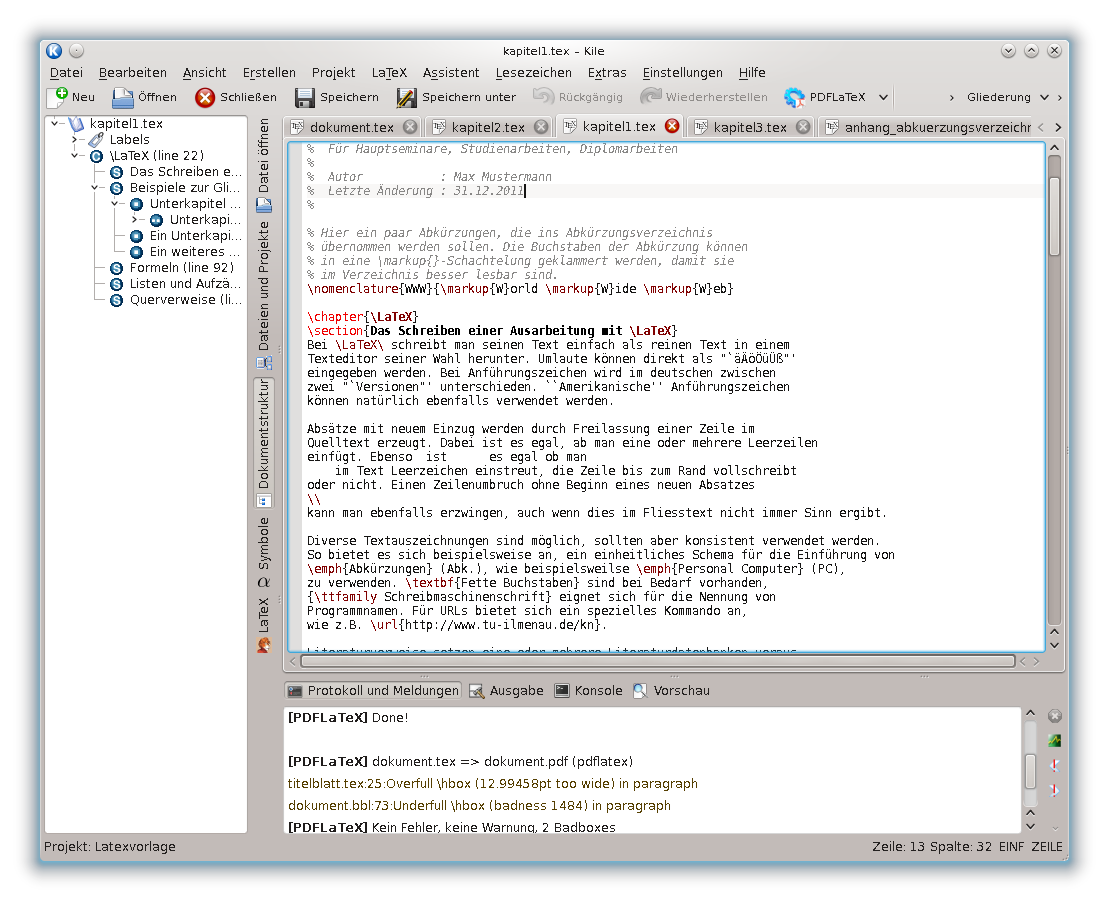
\includegraphics[width=13cm]{bilder/kile_neu.png}
\caption{Bildschirmfoto {\ttfamily kile}}
\label{bild:kile}
\end{figure}

Kile organisiert mehrere Teildokumente zu einem Projekt und
bietet damit einen einfachen Zugriff auf alle Teildokumente
einer Ausarbeitung. Syntaxhighlighting ist ebenfalls vorhanden,
sowohl für \LaTeX als auch für die BibTex"=Literaturdatenbanken.
Für den Start eines \LaTeX"=Durchlaufes sowie den verschiedenen
Konvertierungsmöglichkeiten gibt es einzelne Knöpfe. Ein direktes
Hin- und Herspringen zwischen DVI- und TEX"=Ansicht, wobei
an die korrekte Stelle gesprungen wird, ist möglich. Dies vereinfacht
Korrekturen speziell bei umfangreicheren Dokumenten.



\subsection{{\ttfamily TeXnicCenter} und {\ttfamily TeXworks} -- Windows}
Die \TeX-Entwicklungsumgebungen sind in den Bildschirmfotos \ref{bild:texniccenter} und \ref{bild:texworks} zu sehen.

\begin{figure}[!ht]
\centering
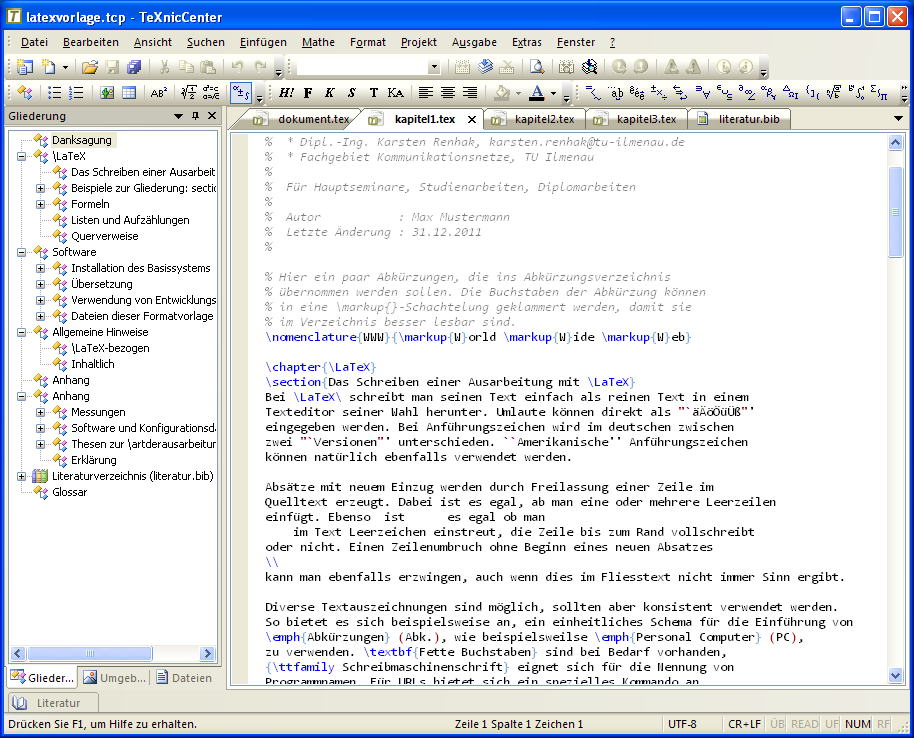
\includegraphics[width=13cm]{bilder/texniccenter_neu.png}
\caption{Bildschirmfoto {\ttfamily TeXnicCenter}}
\label{bild:texniccenter}
\end{figure}

\begin{figure}[!ht]
\centering
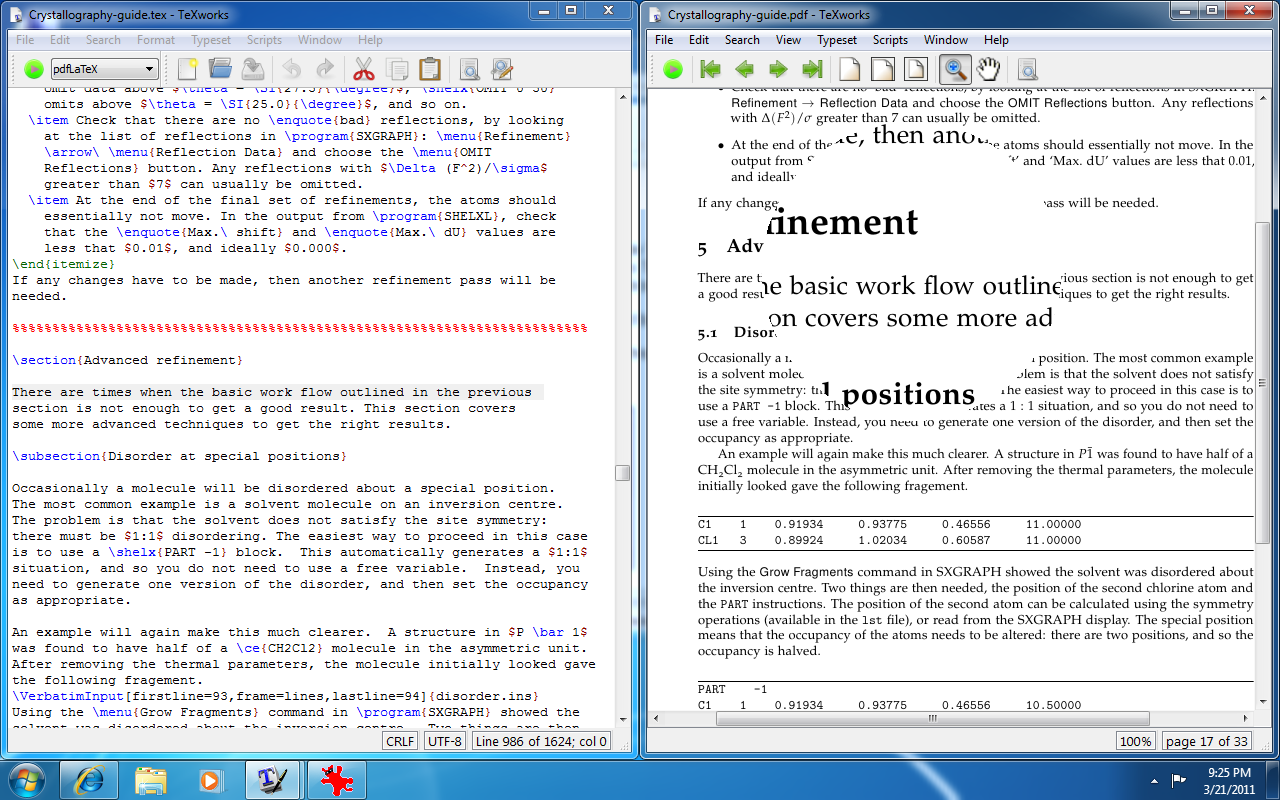
\includegraphics[width=\textwidth]{bilder/texworks-win7.png}
\caption{Bildschirmfoto {\ttfamily TeXworks}}
\label{bild:texworks}
\end{figure}



Beide Editoren bietet Syntaxhighlighting für die verschiedenen
Latexbefehle. Kurz gesagt bieten diese Entwicklungsumgebungen die
selben Features wie die im letzten Abschnitt vorgestellte
Software "`Kile."'

\textbf{Hinweis:} Wenn Sie TeXnicCenter verwenden, nutzen Sie bitte die Version 2.0 (oder größer). Zur Zeit 
(Oktober 2012) ist nur eine Alpha-Version verfügbar. Die TeXnicCenter"=Versionen 1.* unterstützen keine UTF-8 codierten Textdateien. 
Diese Vorlage ist jedoch im UTF-8 Zeichensatz \cite{wiki:utf8} gespeichert.

\nomenclature{UTF}{\markup{U}CS \markup{T}ransformation \markup{F}ormat}
\nomenclature{UCS}{\markup{U}niversal \markup{C}haracter \markup{S}et}


\section{Dateien dieser Formatvorlage}
Siehe Tabelle \ref{tabelle:dateien}.

\begin{table}[ht!]
\centering
\begin{tabular}{ll}
\hline
Dateiname &
Beschreibung
\\
\hline
{\ttfamily abschlusserklaerung.tex} &
\LaTeX\ Teildokument
\\
{\ttfamily anhang\_abbildungsverzeichnis.tex} &
\LaTeX\ Teildokument
\\
{\ttfamily anhang\_abkuerzungsverzeichnis.tex} &
\LaTeX\ Teildokument
\\
{\ttfamily anhang\_literaturverzeichnis.tex} &
\LaTeX\ Teildokument
\\
{\ttfamily anhang\_messwerte.tex} &
\LaTeX\ Teildokument
\\
{\ttfamily anhang\_programm\_a.tex} &
\LaTeX\ Teildokument
\\
{\ttfamily anhang\_programm\_b.tex} &
\LaTeX\ Teildokument
\\
{\ttfamily anhang\_protokoll.tex} &
\LaTeX\ Teildokument
\\
{\ttfamily anhang\_tabellenverzeichnis.tex} &
\LaTeX\ Teildokument
\\
{\ttfamily bilder/} &
Hier alle Bilder ablegen!
\\
{\ttfamily dokument.dvi} &
Ergebnis des \LaTeX\ Durchlaufes
\\
{\ttfamily dokument.pdf} &
Erzeugtes PDF"=Dokument
\\
{\ttfamily dokument.ps} &
Erzeugtes Postscript"=Dokument
\\
{\ttfamily dokument.tex} &
\LaTeX\ Hauptdokument
\\
{\ttfamily itmabbrv.bst} &
Formatvorlage
\\
{\ttfamily itmalpha.bst} &
Formatvorlage
\\
{\ttfamily kapitel1.tex} &
\LaTeX\ Teildokument
\\
{\ttfamily kapitel2.tex} &
\LaTeX\ Teildokument
\\
{\ttfamily kapitel3.tex} &
\LaTeX\ Teildokument
\\
{\ttfamily kurzfassung.tex} &
\LaTeX\ Teildokument
\\
{\ttfamily latexvorlage.kilepr} &
Projektdatei für {\ttfamily Kile}
\\
{\ttfamily latexvorlage.tcp} &
Projektdatei für {\ttfamily TeXnicCenter}
\\
{\ttfamily literatur.bib} &
Die Literaturdatenbank
\\
{\ttfamily thesen.tex} &
\LaTeX\ Teildokument
\\
{\ttfamily titelblatt.tex} &
\LaTeX\ Teildokument
\\
{\ttfamily vorwort.tex} &
\LaTeX\ Teildokument
\\
\hline
\end{tabular}
\caption{Relevante Dateien im Paket}
\label{tabelle:dateien}
\end{table}


%% ++++++++++++++++++++++++++++++++++++++++++++++++++++++++++++
%% Kapitel 3: Allgemeine Hinweise
%% ++++++++++++++++++++++++++++++++++++++++++++++++++++++++++++
%
%  Gerüst:
%  * Version 0.11
%  * Dipl.-Ing. Karsten Renhak, karsten.renhak@tu-ilmenau.de
%  * Fachgebiet Kommunikationsnetze, TU Ilmenau
%
%  Für Hauptseminare, Studienarbeiten, Diplomarbeiten
%
%  Autor           : Max Mustermann
%  Letzte Änderung : 31.12.2011
%

\chapter{Allgemeine Hinweise}
\section{\LaTeX-bezogen}
\begin{description}
\item[Abkürzungsverzeichnis]
      Sollte das Abkürzungsverzeichnis nach dem Hinzufügen eines
      {\ttfamily nomenclature}"=Kommandos nicht aktualisiert werden,
      muss der {\ttfamily makeindex}"=Aufruf
      manuell in der Konsole gestartet werden. Manche
      Entwicklungsumgebungen machen dies aber schon automatisch.
      Bitte die genannten Parameter nicht vergessen!

      Bei Benutzern der GUI \texttt{Kile} kann es vorkommen,
      dass der \texttt{makeindex}-Befehl nicht automatisch ausgeführt
      wird, scheint ein Bug zu sein. In diesem Fall kann der Index
      auch manuell durch Aufruf von \texttt{makeindex} aktualisiert
      werden.
\item[Thesenpapier]
      Für die Thesen wurde mit der Version 0.8 an ein eigenständiges
      Dokument namens {\ttfamily thesen-handout.tex} hinzugefügt.
      Es bindet ebenso wie das Hauptdokument die Datei
      {\ttfamily thesen.tex} ein, erzeugt aber eben nur dieses
      eine Blatt ohne eine Seitenzahl.
\item[Beidseitiger Druck]
      Im Zentraldokument {\ttfamily dokument.tex} kann das Layout
      auf doppelseitigen Druck umgeschaltet werden (Option
      {\ttfamily twoside} statt {\ttfamily oneside}). Allerdings
      verlangen manche Prüfungsämter explizit einen einseitigen
      Druck! Neue Kapitel ({\ttfamily chapter}) beginnen dabei
      automatisch auf einer Vorderseite (\(\to \) rechte Seite).
      Die Ränder sind dabei innen nur halb so breit wie außen, was
      aber Absicht ist: Zusammen ergeben die linke und die rechte
      Seite innen einen "`weißen Streifen"', der genauso breit ist wie die
      äußeren Ränder.
\item[Überlange Kapitelüberschriften]
      Manchmal müssen Überschriften sehr lang sein, sodass sie von \LaTeX\ 
      umgebrochen werden. Dieses Verhalten ist aber weder im Inhaltsverzeichnis
      noch in der Kopfzeile erwünscht! Daher kann man zu einer überlangen
      Überschrift auch eine Kurzform mit angeben, welche dann im Inhaltsverzeichnis
      und im Dokumentenkopf verwendet wird:\\
      {\ttfamily \textbackslash chapter[Kurzform]\{Langform\}}
\item[Einzüge]
      Bitte \emph{nicht!} die Einzüge ändern oder abschalten. Das ist
      so gewollt und verbessert den Lesefluss! (Stichwort
      \texttt{\textbackslash setlength\textbackslash parindent\{0pt\}})!
\item[BibTeX-Einträge mit mehreren Autoren]
      Sollen mehrere Autoren angegeben erden, so sind diese einzeln
      als \emph{Vorname Nachname} anzugeben und durch \texttt{and}
      voneinander zu trennen. BibTeX ersetzt das \texttt{and} dann
      durch das deutsche "`und"':\\
      \texttt{author = \{Adam Riese and Eva Zwerg\},}
\end{description}




\section{Inhaltlich}
\begin{itemize}
\item Überschriften im Inhaltsverzeichnis nie tiefer als
      vier Ebenen. Dies geht mit \LaTeX\ auch gar nicht anders,
      da {\ttfamily subsubsection} bereits die niedrigste
      Schachtelungstiefe darstellt, welche noch im
      Inhaltsverzeichnis aufgeführt wird.
\item Die Kapitel sollten in der späteren Ausarbeitung anders
      benannt werden als in dieser Formatvorlage. Eine Diplomarbeit
      \emph{kann} beispielsweise aus der folgenden Aufteilung bestehen:

      \begin{enumerate}
      \item Problemstellung
      \item Theoretische Grundlagen
      \item Herleitung
      \item Der Prototyp
      \item Zusammenfassung
      \item Ausblick
      \end{enumerate}
\item Es empfiehlt sich, ein Programm zur Rechtschreibprüfung zu
      installieren. Alternativ zu einer \LaTeX"=fähigen
      Rechtschreibkorrektursoftware kann ein Abschnitt auch
      in bspw. Microsoft Word getippt und geprüft werden, bevor
      er dann in das \LaTeX"=Dokument eingefügt wird.
\item Für Diplomarbeiten wird generell ein englischer "`Abstract"'
      benötigt!
\end{itemize}

%\input{kapitel4.tex}
%\input{kapitel5.tex}
%\input{kapitel6.tex}



\appendix
\part*{Anhang}
\chapter{Messungen}
Beispieltext

%% ++++++++++++++++++++++++++++++++++++++++++++++++++++++++++++
%% Anhang: Beispielkapitel "Protokoll"
%% ++++++++++++++++++++++++++++++++++++++++++++++++++++++++++++
%
%  Gerüst:
%  * Version 0.10
%  * Dipl.-Ing. Florian Evers, florian.evers@tu-ilmenau.de
%  * Fachgebiet Kommunikationsnetze, TU Ilmenau
%
%  Für Hauptseminare, Studienarbeiten, Diplomarbeiten
%
%  Autor           : Max Mustermann
%  Letzte Änderung : 31.12.2004
%

\section{Protokoll}
Beispieltext

%% ++++++++++++++++++++++++++++++++++++++++++++++++++++++++++++
%% Anhang: Beispielkapitel "Messwerte"
%% ++++++++++++++++++++++++++++++++++++++++++++++++++++++++++++
%
%  Gerüst:
%  * Version 0.10
%  * Dipl.-Ing. Florian Evers, florian.evers@tu-ilmenau.de
%  * Fachgebiet Kommunikationsnetze, TU Ilmenau
%
%  Für Hauptseminare, Studienarbeiten, Diplomarbeiten
%
%  Autor           : Max Mustermann
%  Letzte Änderung : 31.12.2004
%

\section{Messwerte}
Beispieltext


\chapter{Software und Konfigurationsdateien}
Beispieltext

%% ++++++++++++++++++++++++++++++++++++++++++++++++++++++++++++
%% Anhang: Beispielkapitel "Programm A"
%% ++++++++++++++++++++++++++++++++++++++++++++++++++++++++++++
%
%  Gerüst:
%  * Version 0.11
%  * Dipl.-Ing. Karsten Renhak, karsten.renhak@tu-ilmenau.de
%  * Fachgebiet Kommunikationsnetze, TU Ilmenau
%
%  Für Hauptseminare, Studienarbeiten, Diplomarbeiten
%
%  Autor           : Max Mustermann
%  Letzte Änderung : 31.12.2011
%

\section{Software A}
Beispieltext

%% ++++++++++++++++++++++++++++++++++++++++++++++++++++++++++++
%% Anhang: Beispielkapitel "Programm B"
%% ++++++++++++++++++++++++++++++++++++++++++++++++++++++++++++

\section{Software B}
Beispieltext




% Literaturverzeichnis einbinden
%% ++++++++++++++++++++++++++++++++++++++++++++++++++++++++++++
%% Anhang: Literaturverzeichnis
%% ++++++++++++++++++++++++++++++++++++++++++++++++++++++++++++


% Mit dem Befehl \nocite werden auch nicht im Text zitierte
% aus der Literaturdatenbank mit in das Literaturverzeichnis aufgenommen.
% Ein "\nocite{*}" übernimmt ungeprüft die komplette Datenbank.
%\nocite{*}

\cleardoublepage
\ihead[]{Literaturverzeichnis}
\bibliographystyle{alphadin}
\bibliography{literatur} % "literatur.bib" ist hier die einzige Literaturdatenbank.

% Alternativ: Mehrere Datenbanken verwenden, falls eine
% oder mehrere umfangreiche Sammlungen exisitieren:
%\bibliography{literatur_buecher,literatur_weblinks}


% Abbildungsverzeichnis einbinden

\cleardoublepage
\ihead[]{Abbildungsverzeichnis}
\listoffigures


% Tabellenverzeichnis einbinden
%% ++++++++++++++++++++++++++++++++++++++++++++++++++++++++++++
%% Anhang: Tabellenverzeichnis
%% ++++++++++++++++++++++++++++++++++++++++++++++++++++++++++++

% Hier keine weiteren Änderungen vornehmen
\cleardoublepage
\ihead[]{Tabellenverzeichnis}
\listoftables



% Abkürzungsverzeichnis einbinden
%% ++++++++++++++++++++++++++++++++++++++++++++++++++++++++++++
%% Anhang: Abkürzungsverzeichnis
%% ++++++++++++++++++++++++++++++++++++++++++++++++++++++++++++


% Hier keine weiteren Änderungen vornehmen
\cleardoublepage
\ihead[]{Abkürzungsverzeichnis und Formelzeichen}
\printnomenclature



% Thesen
%% ++++++++++++++++++++++++++++++++++++++++++++++++++++++++++++
%% Thesen zur Ausarbeitung. Für Diplomarbeiten
%% ++++++++++++++++++++++++++++++++++++++++++++++++++++++++++++
%
%  Gerüst:
%  * Version 0.11
%  * Dipl.-Ing. Karsten Renhak, karsten.renhak@tu-ilmenau.de
%  * Fachgebiet Kommunikationsnetze, TU Ilmenau
%
%  Für Hauptseminare, Studienarbeiten, Diplomarbeiten
%
%  Autor           : Max Mustermann
%  Letzte Änderung : 31.12.2011
%

\chapter*{Thesen zur \artderausarbeitung}
\addcontentsline{toc}{chapter}{Thesen zur \artderausarbeitung}
\ihead[]{Thesen zur \artderausarbeitung}

\begin{enumerate}
\item Mit \LaTeX\ gesetzte Dokumente sehen überall
      gleich aus. Sie werden ähnlich wie HTML in Klartext
      geschrieben und anschließend mit Hilfe eines Konverters in
      Postscript- oder PDF"=Dateien gewandelt.
\item \LaTeX\ gibt es für alle wichtigen Betriebssysteme.
\item Die Benutzung einer integrierten Entwicklungsumgebung,
      beispielsweise {\ttfamily Kile} oder {\ttfamily TeXnicCenter},
      wird empfohlen.
\item Dieses Dokument ist Formatvorlage und Einstiegshilfe
      zugleich. Einfach den Text durch die eigene Ausarbeitung
      ersetzen.
\end{enumerate}

% Etwas Platz schaffen:
\section*{}

Ilmenau, den 31.\,12.\,2011\hfill \namedesautors


% Abschlusserklärung

\chapter*{Erklärung}
\addcontentsline{toc}{chapter}{Erklärung}
\ihead[]{Erklärung}

Die vorliegende Arbeit habe ich selbstständig ohne Benutzung anderer als der
angegebenen Quellen angefertigt. Alle Stellen, die wörtlich oder sinngemäß
aus veröffentlichten Quellen entnommen wurden, sind als solche
kenntlich gemacht. Die Arbeit ist in gleicher oder ähnlicher Form oder
auszugsweise im Rahmen einer oder anderer Prüfungen noch nicht vorgelegt
worden.
\\[2cm]
Ilmenau, den 15.\,07.\,2020\hfill \namedesautors


\end{document}

